\begin{figure}[t]
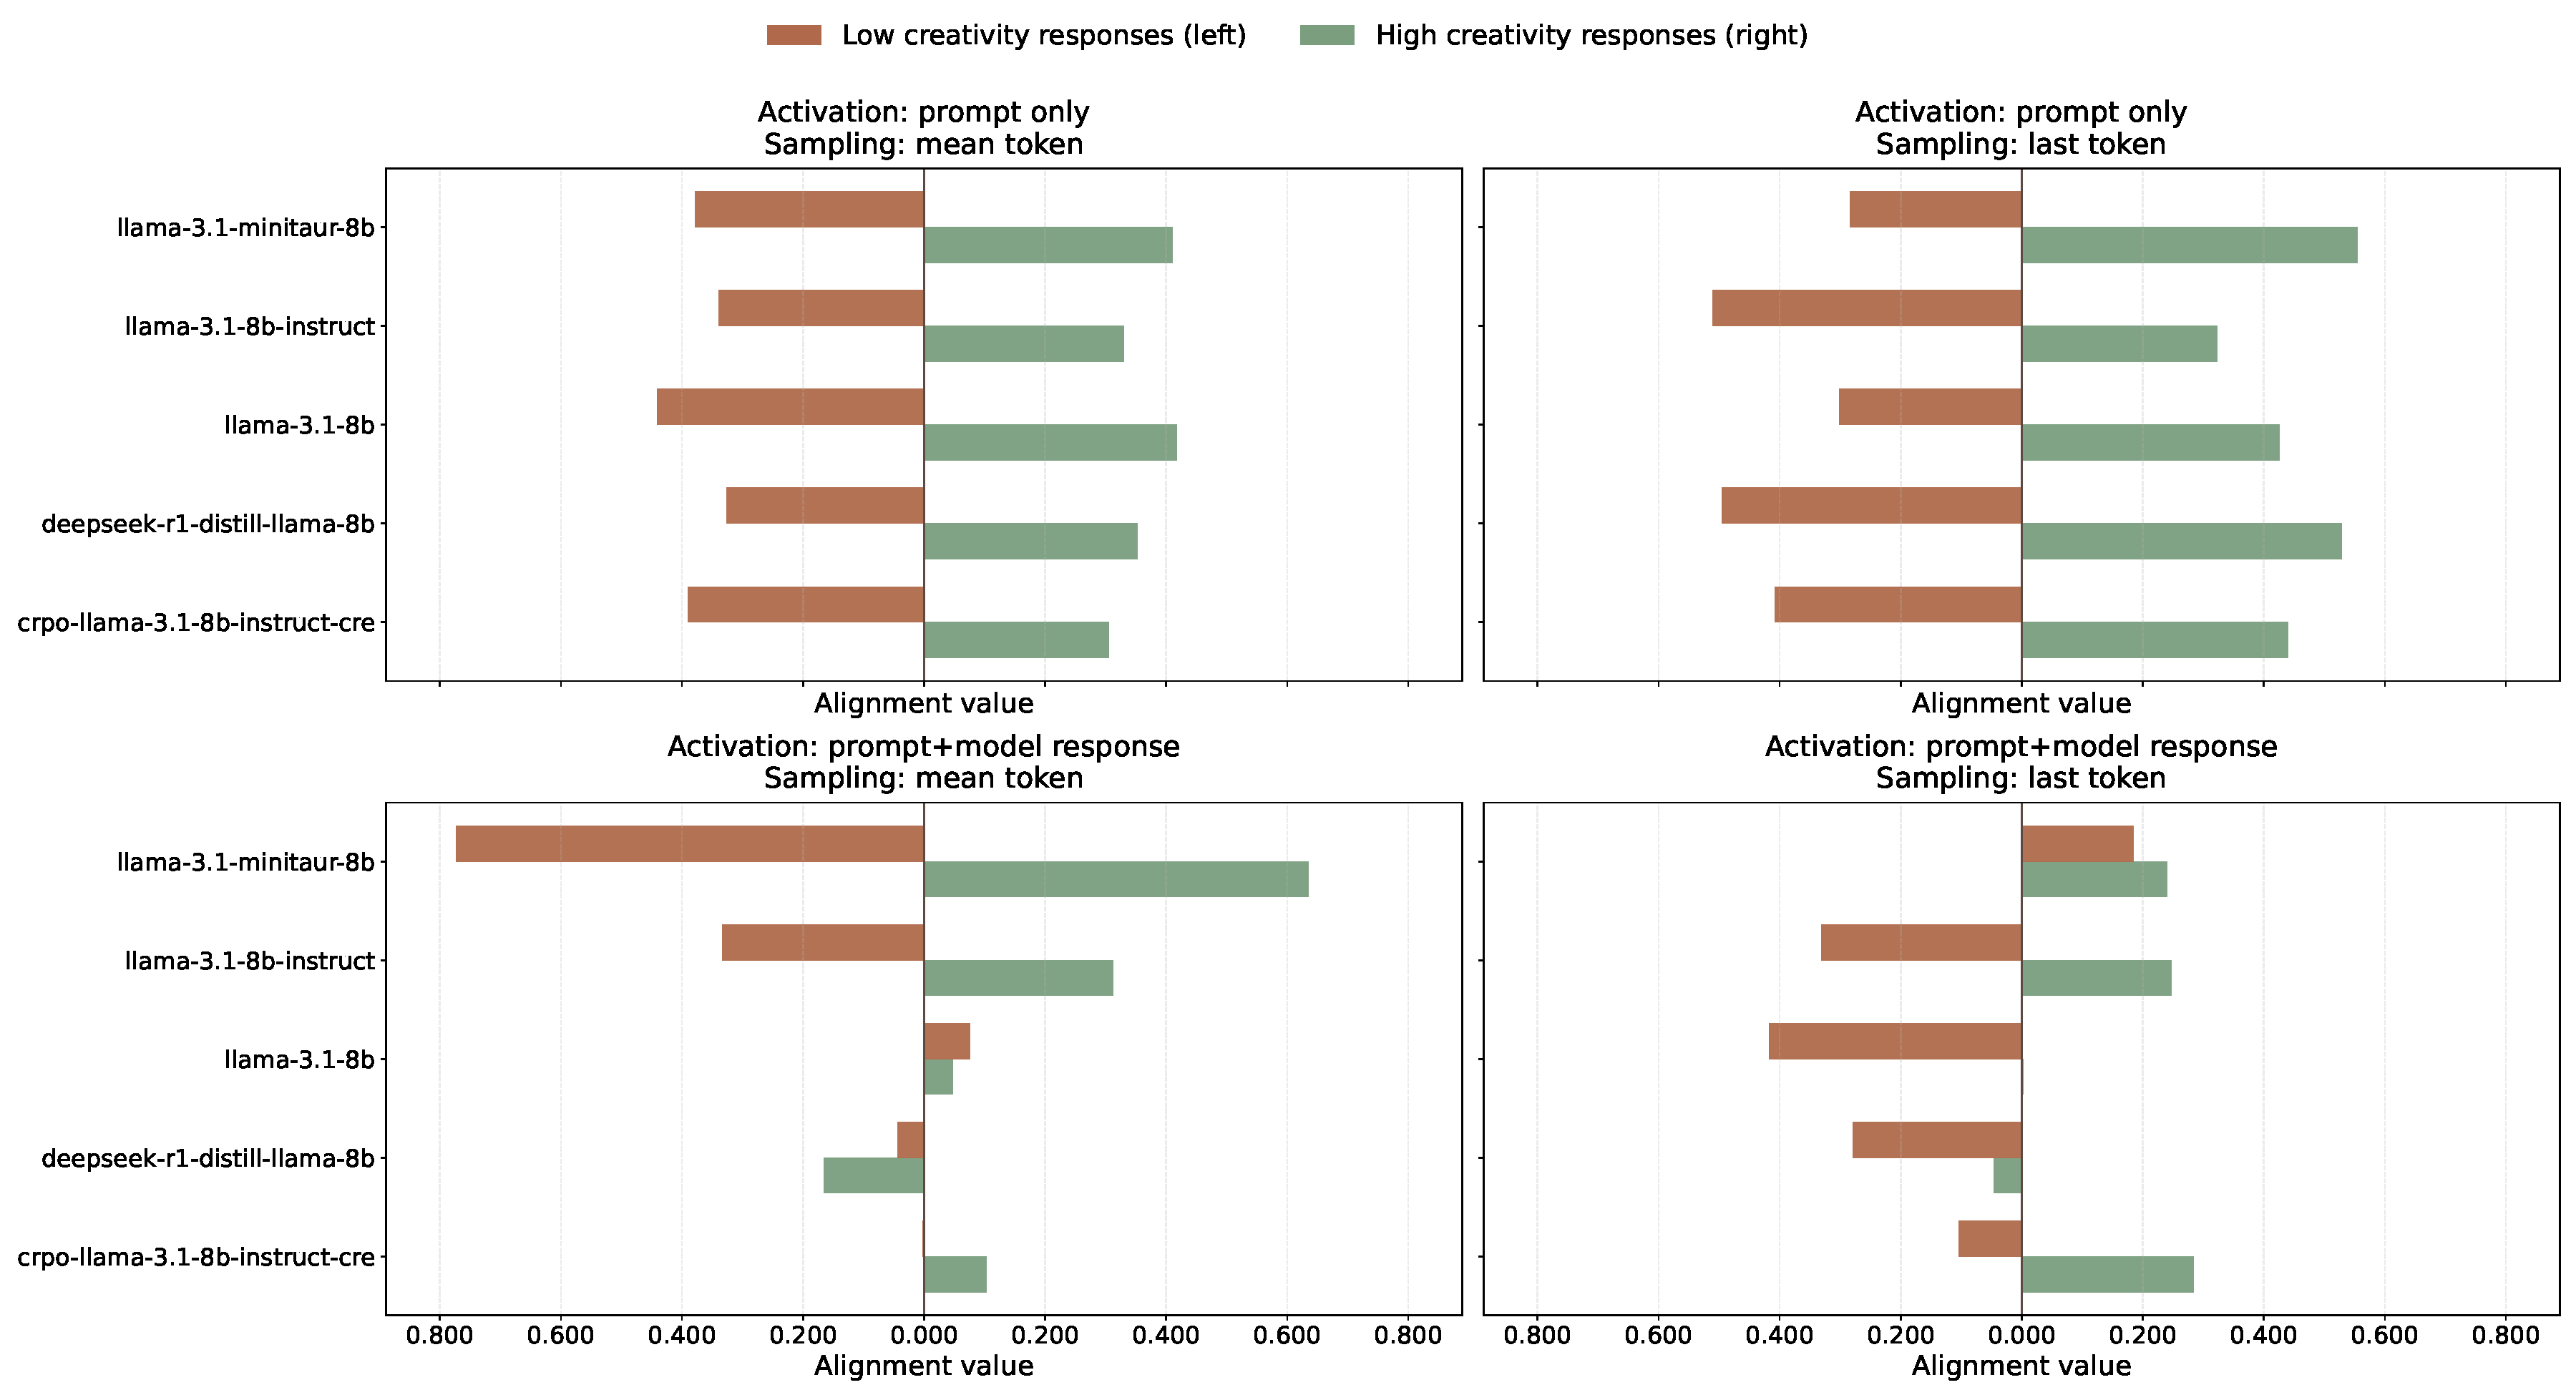
\includegraphics[width=\linewidth]{figures/high_low_cre_comparison_nc0.0.pdf}
\centering
\caption{\textbf{Default Mode Network (DMN) AUT brain alignment results for high and low creativity response populations.} The left red and right green bars indicate positive alignment with high and low creativity responses, respectively. Flipped bars indicate negative alignment.}
\label{fig:alignment-high-low}
\end{figure}

\paragraph{LLMs Align with the Human Brain During Creative Thinking}
Figure \ref{fig:alignment-aut-yeo-dmn-prompt} shows the brain alignment between the Default Mode Network (DMN) and model representations extracted during early cue processing — that is, after the prompt has been presented but before any response has been generated. Notably, the DMN has been directly implicated in creative cognition and is considered a core neural substrate of creative thinking \citep{luchini2025role}. We observe moderate and consistent alignment across models, and crucially, this \textbf{alignment is positively correlated with both model size} ($r=0.58, p<0.05$) and \textbf{creative task performance} as measured by the AUT score ($r=0.51, p<0.05$). This suggests that larger and more creatively capable models more closely mirror the neural representations underlying human divergent thinking during the initial stages of ideation. However, when alignment is measured using representations extracted after the model has generated its response, alignment values become more variable across models, and the correlations with both model size and task performance weaken (Appendix Figure \ref{fig:alignment-aut-yeo-dmn-response}). This decoupling may reflect the fact that models tend to converge on similar responses regardless of scale \citep{wenger2025we, ismayilzada2024evaluating}, or alternatively, that generated responses increasingly diverge from human responses in length, structure, and quality as model scale grows. We also replicate some of these patterns (i.e. correlation with AUT score) for the Frontoparietal Network (FPN) (See Appendix Figures \ref{fig:alignment-aut-yeo-fp-prompt} and \ref{fig:alignment-aut-yeo-fp-response}). To assess whether these effects are specific to creative cognition or reflect more general properties of model or brain representations, we repeat the alignment analyses using the non-creative OCT task and a brain network not typically associated with creativity, namely the Somatomotor network \citep{ji2019mapping}. As shown in Appendix Figures \ref{fig:alignment-oct-model-size-yeo-dmn} and \ref{fig:alignment-aut-yeo-som-prompt}, neither model size nor task performance correlates significantly with alignment in either of these conditions, providing an important double dissociation that strengthens the interpretation that the observed alignment effects are driven specifically by the conjunction of a creativity-relevant task and a creativity-relevant brain network.

\paragraph{Higher Layers of LLMs Show Stronger Alignment with Creative Brain Responses}
A well-established finding is that different layers of a model capture qualitatively different aspects of linguistic and cognitive processing: earlier layers tend to encode core syntactic and lexical properties, while later layers are associated with higher-level, task-specific representations involving reasoning and cognition \citep{tenney2019bert, jawahar-etal-2019-bert}. Given that creative thinking is itself a higher-order cognitive process, we hypothesized that deeper layers of LLMs would show preferentially stronger alignment with brain responses during the AUT task. To investigate this, we visualize the distribution of the relative layer depth (Figure \ref{fig:alignment-best-layer-aut-yeo-dmn}) at which peak alignment is achieved across models (defined as the best layer index divided by the total number of layers), and compute its correlation with alignment predictivity. As shown in Figure \ref{fig:alignment-best-layer-aut-yeo-dmn}, we find a significant positive correlation between relative layer depth and alignment ($r=0.54, p<0.05$), indicating that brain alignment during creative thinking is predominantly driven by the higher-level representations of LLMs rather than early-layer processing. This is consistent with the view that the neural geometry of divergent thinking is more closely mirrored by the abstract, task-sensitive representations that emerge in the later stages of model computation \citep{caucheteux2022brains}.

\paragraph{Post-Training Objectives Differentially Modulate Alignment with High- and Low-Creativity Neural Responses}
To investigate the effects of different post-training approaches, we partition the brain data into high and low creativity populations as described in Section \ref{sec:high-low} and measure brain alignment separately for each population across several variants of the \texttt{Llama-3.1-8B} model as described in Section \ref{sec:models}. The results are shown in Figure \ref{fig:alignment-high-low}. During early prompt processing, all model variants show broadly comparable alignment with both populations. However, once models begin generating responses, the alignment dynamics diverge markedly across training conditions. Most notably, comparing \texttt{Llama-3.1-8B-Instruct} with its creativity-optimized counterpart \texttt{CrPO-Llama-3.1-8B-Instruct}, we find that while the instruct model maintains similar alignment with both populations, the CRPO model shows a significant decrease in alignment with low-creativity responses while preserving moderate alignment with high-creativity responses, a targeted shift consistent with the model's training objective. The base pretrained \texttt{Llama-3.1-8B} largely loses alignment in the response generation stage, likely due to its inability to follow task instructions. In contrast, \texttt{Llama-3.1-Minitaur-8B}, which is fine-tuned to predict and simulate human behavior, shows elevated alignment with both populations during response generation, plausibly reflecting its closer correspondence to human response patterns. Finally, \texttt{DeepSeek-R1-Distill-Llama-8B}, the base model fine-tuned with reasoning chains distilled from DeepSeek-R1, exhibits a striking reversal: negative alignment with high-creativity responses and positive alignment with low-creativity responses, suggesting that chain-of-thought reasoning training steers model representations away from the neural geometry of creative ideation and toward more systematic, analytical processing.